\documentclass{article}

% Language setting
% Replace `english' with e.g. `spanish' to change the document language
\usepackage[english]{babel}

% Set page size and margins
\usepackage[letterpaper,top=2cm,bottom=2cm,left=3cm,right=3cm,marginparwidth=1.75cm]{geometry}
% Useful packages
\usepackage{amsmath}
\usepackage{graphicx}
\usepackage{minted}
\usepackage[colorlinks=true, allcolors=blue]{hyperref}

\title{Homework 2 \\ Language Based Technology for Security} 
\author{Niccolo' Piazzesi \\ n.piazzesi@studenti.unipi.it}

\begin{document}
\maketitle
\frenchspacing

\section{Introduction}
For this homework, i will present and discuss the paper "\textbf{MirChecker: Detecting Bugs in Rust Programs via Static Analysis}" by 
Zhuohua Li, Jincheng Wang, Mingshen Sun, and John C.S Lui \cite{li2021mirchecker}. This paper presents a novel static analysis tool for the Rust programming language, 
focusing on detecting and preventing potential runtime crashes and memory safety bugs.
\section{Paper Summary}
We can divide the paper in five parts: at the beginning, all the necessary background knowledge about static analysis and Rust 
is established, and the main motivations for the tool development are explained. Then, the high level design of the tool is presented, and the reasoning behind all the relevant choices is 
given. After that, the authors delve deeper in the actual implementation, showing the algorithm used and giving all the important technical details. The last part is about a series of benchmark used to 
test both the efficacy and speed of the developed tool on target examples. Finally, the authors discuss the achieved results, limitations, and the potential future directions of their work.
\subsection{Background Knowledge and Motivations}
The paper begins by giving the basic knowledge needed to understand its results. The authors start by presenting all the necessary  theory and concepts of abstract interpretation. 
They recall the notions of \textbf{lattice} and \textbf{abstract transfer functions}, showing how they are  used to represent computations on abstract program states. 

In the next part, there is an introduction on the  main features of Rust, mainly about its 
powerful type and ownership system. It is mentioned how the restrictive rules for aliasing and mutability prevents many of the typical memory corruption problems. After, the main motivation for the work is presented: although 
Rust has very advanced tools for memory safety, their incomplete nature and the presence of the \mintinline{rust}{unsafe} keyword  can breach its safety promises, leading  to undetected bugs or worse, undefined behavior. The paper focuses on two 
classes of issues affecting the language: \begin{itemize}
    \item \textbf{Runtime panics}.  Rust's type system cannot enforce all the security conditions statically. Some conditions such as array bounds checking or integer overflow detection are postponed until execution, with 
    the compiler automatically instrumenting assertions that, when violated, halt the program. Although this is still a safe way to handle these issues (no memory corruption is possible), an attacker could still exploit this 
    to cause denial of service.
    \item \textbf{Lifetime corruptions.} While  classical memory corruption bugs such as use-after-free or dangling pointers are well managed in Rust, using \mintinline{rust}{unsafe} and combining 
    it with the ownership system may lead to lifetime bugs where, first the unsafe code  causes invalid pointers or shared mutable memory, and then the ownership system automatically drops that memory, leading back to use after free bugs.
\end{itemize}
To prevent these issues, the authors decided to combine numerical static analysis to detect possible runtime panics generated by integer operations,
 and symbolic analysis to track heap memory ownership.
\subsection{High level design}
MirChecker performs static analysis on top of Rust's Mid-level Intermediate Representation (MIR). MIR is produced as an intermediate step during normal compilation. 
It corresponds to a control flow graph (CFG) representation  and borrow checking is performed on it. Traditionally, Rust static analysis tools reason on LLVM IR or  a custom IR, but the authors decided to use MIR 
for two main reasons. First, while it reduces most of the complex syntax to a simpler core language, it preserves type information and debugging data, which is used to simplify the actual algorithm.
Second, LLVM API targets directly C/C++ and is then ported to Rust. Many compatibility issues may arise, differently from using 
a native representation. 


\paragraph{User interface} MirChecker is shipped as a subcommand of  
Cargo, Rust's official package manager. This makes it possible to reuse the entire
Rust compiler toolchain for dependency resolving. Dependency information is used 
to distinguish between source files in the current crate (crates are how packages in Rust are called) and dependencies, which are ignored 
by MirChecker for efficiency purposes. Tool invocation is highly customizable, with many options 
to control the behavior of the analysis. Some of the options are shown in \autoref{mir-cli}.
\begin{figure}[H]
\begin{minted}{bash}
    cargo mir-checker --\ 
    --entry <entry-function-name>\
    --domain <abstract-domain>\ 
    --widening_delay <N>\
    --narrowing_iteration <N>\ 
    --suppress_warnings <S>
\end{minted}
    \caption{MirChecker example invocation}
    \label{mir-cli}

\end{figure}


\paragraph{Static analyzer}
The analyzer is implemented as a custom callback function for the Rust compiler, and is 
automatically called after all the necessary data structures are built. 

The actual algorithm uses standard techniques from Abstract Interpretation.
The CFG is first preprocessed to create a topological ordering of the basic blocks. After, the algorithm traverses the CFG according to the ordering 
and iteratively executes \textit{Abstract Interpretation} until the result reaches a fix point.
In the following step, several bug detectors are called. These bug detectors use 
constraint solving techniques to determine if some security conditions are violated or not. At the end, a series of 
diagnostics are emitted to the users, leveraging the compiler infrastructure to provide clear and informative messages.
\autoref{fig:hilev} provides a visualization of the entire process.
\begin{figure}[H]
    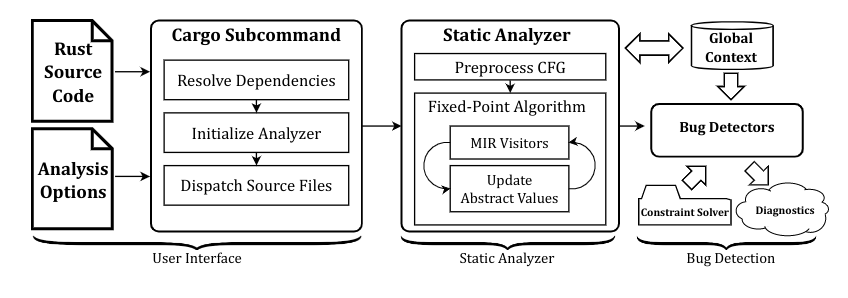
\includegraphics[scale=0.5]{hilev.png}
    \caption{High level view of Mir-Checker architecture}
    \label{fig:hilev}
\end{figure}
\subsection{Implementation}

\subsubsection{Abstract Interpretation}
\paragraph{Language model}
The internal language of MirChecker is shown in \autoref{fig:lang}. It is a simplified version of 
MIR, capturing only the relevant aspect for the analysis, namely integer and memory operations. 
\begin{figure}[h]
    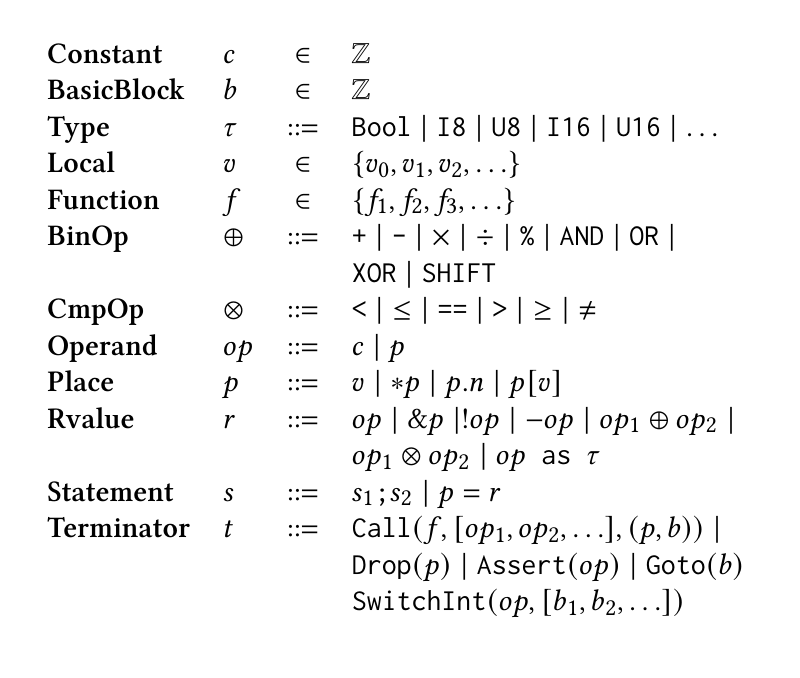
\includegraphics[scale=0.3]{lang.png}
    \caption{MirChecker language model}
    \label{fig:lang}
\end{figure}

The tool reads a program consisting of several functions (global variable initialization is treated as a function as well), and for each of them, builds the 
CFG. A CFG is made of basic blocks, which are the nodes of the graph. At the end of each node there is a \textbf{terminator}, which represents a jump  in the control flow. 
Each terminator is connected with the target block of the jump by an edge in the CFG. There  are five possible terminators:
\begin{itemize}
    \item A $\mathbf{Call(f , [op_1, op_2,...], (p, b))}$ represents a function call taking 
    $op_1,op_2,...$ as arguments and assigning the return value to place $p$ in block $b$.
    \item $\mathbf{Goto(b)}$ represents an unconditional jump to block $b$.
    \item $\mathbf{Drop(p)}$ deallocates  memory  allocated at place $p$.
    \item $\mathbf{Assert(op)}$ continues execution if $op$ evaluates to true, triggering a runtime panic otherwise.
    \item $\mathbf{Switchint(op,[ b_1, b_2, ...])}$ is the symbolic representation of a conditional jump.
    

\end{itemize}
\paragraph{Memory model} The memory model is simple but rigorous. When a \textbf{Place} is accessed 
in a block, a symbolic expression is constructed and used as an abstract memory address. This expression represents a key of the memory lookup 
table. Two expressions are considered equivalent by syntactical comparison. This design can lead 
to a significant loss of precision, which is mitigated by reducing the symbolic expressions with the 
rules shown in \autoref{fig:reduction}. This simplification is caused by the fact that MIR actual memory model is pretty complex as it is still 
a high level intermediate representation, opposed to the load/store model used by LLVM IR in the following compilation stages.

\begin{figure}[H]
    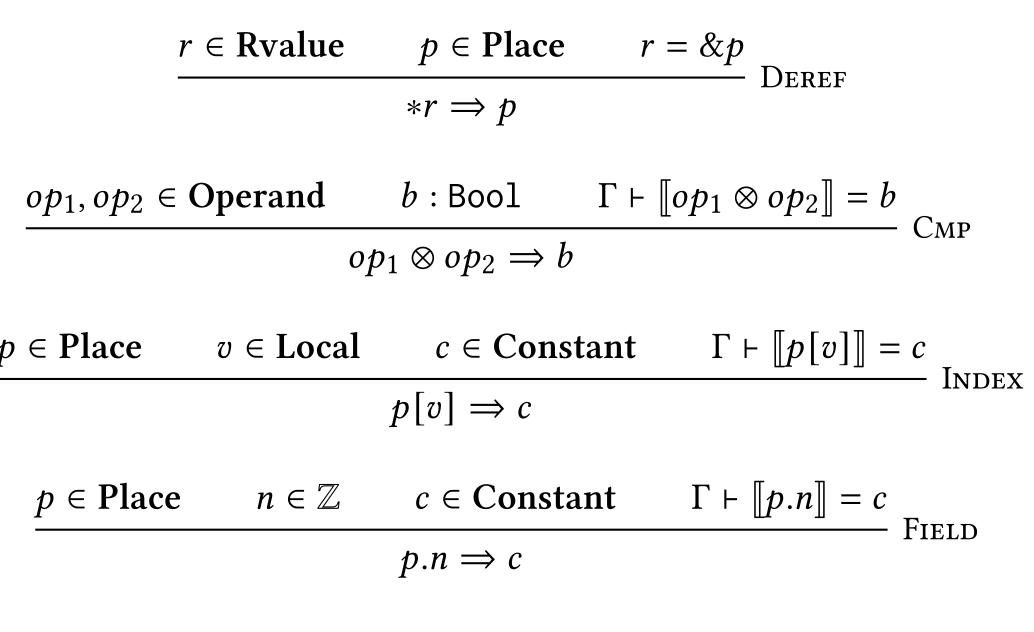
\includegraphics[scale=0.3]{red.png}
    \caption{Reduction rules}
    \label{fig:reduction}
\end{figure}
\paragraph{Abstract domains}
Let \textbf{P} be the set of places  occurring in a CFG, MirChecker maintains a lookup table $\sigma_b : P \rightarrow V$, mapping each place 
to its abstract value. The set \textbf{V} is the set of all possible abstract values and is defined as a 
\textit{lattice} with $\bot$ and $\top$ representing no value and all possible values. There are two categories of values inside \textbf{V}: 
\begin{itemize}
    \item Numerical values (NV) are any integer constraint representation found in 
    classic Abstract Interpretation, mainly intervals, octagons, and polyhedra.
    \item Symbolic values (SV) represent a set of possible values in the right hand side of an assignment. The syntax is defined
    according to the \textbf{Rvalue} in \autoref{fig:lang}. They model  all MIR manipulations that cannot be easily modeled 
    with integer bound constraints, such as references, pairs, indices.
\end{itemize}

The abstract state of computation \textbf{AS} is defined as the \textit{map lattice} of functions from 
\textbf{P} to \textbf{V}. The abstract domain \textbf{AD} is defined as the \textit{map lattice} of functions from the set \textbf{B} of basic blocks to 
\textbf{AS}. Each statement inside a block defines a \textit{transfer function}
that takes as input the abstract state  immediately before the statement, and outputs the abstract state immediately after. The function behavior follows 
the language model abstract semantics.
\paragraph{Numerical and symbolic analysis}
When a transfer function analyze a statement, it first distinguishes 
 the operation should be handled numerically or symbolically  using the different semantics:
\begin{itemize}
    \item If a statement is as an assignment with an integer right hand side, a binary arithmetic operation, or a negation, the left 
    hand side is handled numerically.
    \item For any other statement, a symbolic expression is constructed and stored in the symbolic domain. Reduction rules are applied 
    to simplify each expression.
\end{itemize}
\subsubsection{Algorithm}
The algorithm is divided in four parts: \begin{itemize}
    \item \textbf{CFG traversal}. MirChecker traverses the CFG and iteratively computes a fix point of the abstract values. 
    Intuitively, the algorithm should follow the topological ordering of the basic blocks in a CFG. But the CFG may have loops and as such, not have a 
    well-defined ordering of blocks. The solution is to generalize, using a strategy called \textit{weak topological ordering} (WTO). The input CFG 
    is sorted according to the WTO, which produces a list  of topologically sorted \textit{strongly connected components} (SCC) in the CFG. Each SCC is either 
    a single basic block , or a list of SCC, meaning a loop in the CFG. For simple basic blocks, the algorithm updates the abstract values according to the language model 
    seen before. In the case of a loop, the MIR visitor traverses it repeatedly until a fix point is reached. To ensure that a fix point is always reached, 
    a technique called \textit{widening and narrowing is used}.  If the number of iterations exceeds a certain value, the variable 
    is "widened" to its maximum, and progressively narrowed for several iterations  to get better precision. At the end of each block, the terminator is evaluated, 
    generating further constraints that make the numerical analysis more precise.
    \item \textbf{Interprocedural analysis}. When a function call is made, MirChecker analyzes if the function 
    location can be statically determined. Otherwise, if it is from a dependency or 
    is looked up at runtime (dynamic dispatch through trait objects), the call is simply ignored. 
        The algorithm exploits compiler internals to retrieve 
    type information of the arguments passed to the call and handles context switching and changes in the caller environment. To simplify the analysis, a series 
    of special handlers for commonly used functions that are hard to analyze are provided. Recursive calls are simply skipped, 
    with the visitor stopping after the first call.
    \item \textbf{Verification conditions for bug detections.} After the fix point is reached,  
    the bug detection phase starts. The detectors use information from the abstract domains and verify security conditions
    using Satisfiability Modulo Theories (SMT) solving. Diagnostics messages are produced if a potential bug is found. The detectors 
    can verify \textbf{runtime panics} and \textbf{lifetime corruptions}. Runtime panics conditions 
    are provided by the \textit{Assert(cond)} terminators. The abstract values are translated into SMT formulas 
    that are then evaluated by an appropriate solver. For lifetime corruption, MirChecker maintains an internal 
    list of unsafe functions like \mintinline{rust}{Vec::raw_from_parts}. The symbolic analysis gathers the ownership transfer made by these unsafe functions and checks whether the original owner is used 
    after the ownership was transferred.
    \item \textbf{Eliminating dead variables}. The lifetime of each variable is explicitly encoded by the statements 
    StorageLive and StorageDead inside MIR. The analyzer takes advantage of this to safely cleanup storage without having to perform 
    live variable analysis.
\end{itemize}
\subsubsection{Concrete implementation and external dependencies}

MirChecker is implemented in Rust as a customized callback of the compiler.  It uses three external dependencies: \begin{itemize}
    \item APRON is an abstract domain C library, and it is used to define  the various numerical domains. Since it is a C library, 
    a thin wrapper to define  bindings using  Rust's FFI was needed.
    \item GMP, a GNU library to define arbitrary precision integers. 
    \item Z3, Microsoft's SMT solver. The bug detectors were all defined by using Z3 API bindings for Rust.
\end{itemize}
\subsection{Benchmarks}
MirChecker  was thoroughly tested both in precision and efficiency. The evaluation was performed
in two steps. First, it was evaluated in a "supervised" environment, testing its capacity on a synthetic dataset 
containing well known bugs. All the bugs (4 memory safety bugs, 6 runtime panics) were successfully detected. 

In the second phase, 
MirChecker ability was judged in real life situations. A group of actual Rust crates was collected, with the requirement of having related code to 
the tool itself. This meant collecting crates that perform integer arithmetic and/or use unsafe Rust. The results were pretty interesting: the tool managed to find
17 real runtime panics and 16 real memory-safety problems. 

On the bad side, it was noticed that most of the detected problems 
were false positives. Although this is expected in static analysis, in order to have
a more reliable analysis, an option to suppress specific classes of warnings was implemented. It should be mentioned that, even after warning suppression, there were two outliers (the \textbf{brotli} and \textbf{runes} crates) where the rate 
of false positives stayed at 95\%.

\paragraph{Efficiency} In terms of efficiency, MirChecker was measured both in time and peak memory usage. It was observed that 
the main factor affecting performance is the number of security conditions checked, especially numerical conditions. The choice of the numerical abstract domain 
was found to be the critical tradeoff between efficiency and precision. Interval and linear congruence  consumed less resources but were not as precise as constraint-based domains 
like octagon and polyhedra, which in turn required more memory and time. Another aspect tested was  the dead variable cleaning mechanism 
employed by MirChecker. It was measured to improve performance by 
 10-15\% for constraint-based domains,  while having no major effect for linear congruence and interval domains. 
 
 \section{Advantages}

 \paragraph{Cargo integration} I think that integrating a static analysis tool inside a language toolchain is a great idea. 
 Static analysis can benefit a lot from compilation information, as demonstrated by MirChecker dead variable analysis or its 
 informative error messages. Other than that, it favours adoption by end users, who can benefit from the additional checks without 
 having to modify their familiar workflow.


 \paragraph{Using Z3 for bug detection} The authors decided to use Z3 for the bug detection phase. I think this is a 
 strong point of their work. Z3 is a powerful and industry tested SMT solver, featuring many different theories such as integer 
 arithmetic,bit-vectors, uninterpreted functions and many others. By using this power, MirChecker can detect many bugs by simply 
 converting its internal assertions to a Z3 formula and "outsourcing" the actual solving. Not only does this makes the bug solving more robust, 
 it significantly simplifies MirChecker design, which can be focused on optimizing the fix point algorithm, instead of having to add a custom internal solver.

 \paragraph{Type of bugs detected} Rust is a safe language, and as such does not suffer from the typical memory bugs or unexpected crashes. But, as demonstrated in the paper, 
 it can still have various issues that are not natively captured by the type system. I find that the work proposed is extremely valuable in this regard. The bugs addressed by MirChecker
 are hard to manually detect, especially those that arise from an incorrect usage of \mintinline{rust}{unsafe}. Automating their recognition can improve to a great extent code safety, in situations 
 where it is most required.
\section{Disadvantages}

\paragraph{Memory model}
The memory model is, by admission of the authors, lightweight and syntax driven. MirChecker may distinguish 
two  equivalent expressions used as memory addresses simply because the are syntactically different. This makes the analysis 
less precise, and it forced the authors to employ the reduction rules seen before to try and mitigate the issue. The development of an improved
memory model, maybe adapting known formal models  (e.g the concept of heaplets in separation logic \cite{o2019separation}), should be a top priority to  
increase the power of the analysis.

\paragraph{Ignoring Rust advanced features}
For simplicity, MirChecker does not check more advanced features of rust such as dynamic dispatch, concurrent code and many others. While 
this is understandable from a complexity point of view, i think it hinders the analyzer power and convenience. This is true especially for concurrency, 
where problems like deadlocks when using \mintinline{rust}{Mutex<T>}, or data races inside unsafe code could be prevented 
using automatic detection.

\section{Possible Improvements}

\paragraph{Increasing the number of problems checked}
Right now MirChecker checks only integer operations and possible lifetime issues. 
A first improvement would be to extend the range  of bugs detected. For example, the overflow 
analysis could be extended to floating point operations, which could be extremely valuable 
to analyze math-intensive crates such as \textbf{ndarray} or \textbf{nalgebra}.

\paragraph{Refinement}
To mitigate the problem of false positives, the authors could employ a refinement mechanism. Refinement techniques are used to solve 
this exact problem in abstract interpretation \cite{gulavani2006counterexample}\cite{bogomolov2017counterexample}, and they work by iteratively "concretizing" an abstract domain  until it is precise enough. 
How much is "enough" depends on the context, and it might be a configurable parameter of MirChecker.
\paragraph{Under-approximation instead of over-approximation}
A high level improvement  on the general approach used could be made. Citing the authors, "our goal is to provide a useful bug detection tool rather
than enforcing rigorous formal verification.". This is kind in contrast with the over-approximation technique used in the algorithm. Recent developments 
in the formal methods community \cite{o2019incorrectness}\cite{murray2021incremental}\cite{le2022finding} have shown that using an under-approximation perspective can benefit bug detection. Losing soundness but gaining only true positive  alerts 
is a tradeoff that might be beneficial in this context.
\bibliographystyle{unsrt}
\bibliography{bib.bib}
\end{document}